%% start of file `template.tex'.
%% 
%% Original Copyright 2006-2013 Xavier Danaux (xdanaux@gmail.com).
%% Modified Copyright 2021-2022: Rajib Das Bhagat (rajibdasbhagat@gmail.com).
%
% This work may be distributed and/or modified under the
% conditions of the LaTeX Project Public License version 1.3c,
% available at http://www.latex-project.org/lppl/.


\documentclass[11pt,a4paper,sans]{moderncv}        % possible options include font size ('10pt', '11pt' and '12pt'), paper size ('a4paper', 'letterpaper', 'a5paper', 'legalpaper', 'executivepaper' and 'landscape') and font family ('sans' and 'roman')

\usepackage[utf8]{vietnam}

% moderncv themes
\moderncvstyle{banking}                            % style options are 'casual' (default), 'classic', 'oldstylef' and 'banking'
\moderncvcolor{black}                                % color options 'blue' (default), 'orange', 'green', 'red', 'purple', 'grey' and 'black'
%\renewcommand{\familydefault}{\sfdefault}         % to set the default font; use '\sfdefault' for the default sans serif font, '\rmdefault' for the default roman one, or any tex font name
%\nopagenumbers{}                                  % uncomment to suppress automatic page numbering for CVs longer than one page

% character encoding
\usepackage[utf8]{inputenc}                       % if you are not using xelatex ou lualatex, replace by the encoding you are using
%\usepackage{CJKutf8}                              % if you need to use CJK to typeset your resume in Chinese, Japanese or Korean
\usepackage{fontawesome}
% adjust the page margins
\usepackage[scale=0.9]{geometry}
%\setlength{\hintscolumnwidth}{3cm}                % if you want to change the width of the column with the dates
%\setlength{\makecvtitlenamewidth}{10cm}           % for the 'classic' style, if you want to force the width allocated to your name and avoid line breaks. be careful though, the length is normally calculated to avoid any overlap with your personal info; use this at your own typographical risks...


% personal data
\name{Nguyễn Văn Lộc}{(Nguyen Van Loc)}
\title{Student}
\insti{University of Science, Vietnam National University Ho Chi Minh City}
%\extrainfo{Placement Registration Number: Y/33/CS/20/067}
\address{Place: VNUHCM Dorm B}{Thu Duc}{Ho Chi Minh City, Vietnam}
% optional, remove / comment the line if not wanted; the "postcode city" and and "country" arguments can be omitted or provided empty
\phone[mobile]{+84-905481342}                   % optional, remove / comment the line if not wanted
%\phone[fixed]{+2~(345)~678~901}                    % optional, remove / comment the line if not wanted
%\phone[fax]{+3~(456)~789~012}                      % optional, remove / comment the line if not wanted
\email{vanloc1808@gmail.com}                               % optional, remove / comment the line if not wanted
\homepage{linkedin.com/in/vanloc1808/}                         % optional, remove / comment the line if not wanted

\extrainfo{\homepagesymbol \httplink{github.com/vanloc1808}}
                % optional, remove / comment the line if not wanted
% \photo[64pt][0.4pt]{logo.png}                       % optional, remove / comment the line if not wanted; '64pt' is the height the picture must be resized to, 0.4pt is the thickness of the frame around it (put it to 0pt for no frame) and 'picture' is the name of the picture file
%\quote{Love thy journey, never thy destination!}                           
%----------------------------------------------------------------------------------
%            content
%----------------------------------------------------------------------------------
\begin{document}
%\begin{CJK*}{UTF8}{gbsn}                          % to typeset your resume in Chinese using CJK
%-----       resume       ---------------------------------------------------------
%\makecvtitle
\hypersetup{
    linkcolor=blue,
    filecolor=magenta,      
    urlcolor=cyan,
}
\urlstyle{same}

\noindent
\begin{minipage}{.78\textwidth}
 \makecvtitle
\end{minipage}%
\begin{minipage}{.30\textwidth}
  \centering
  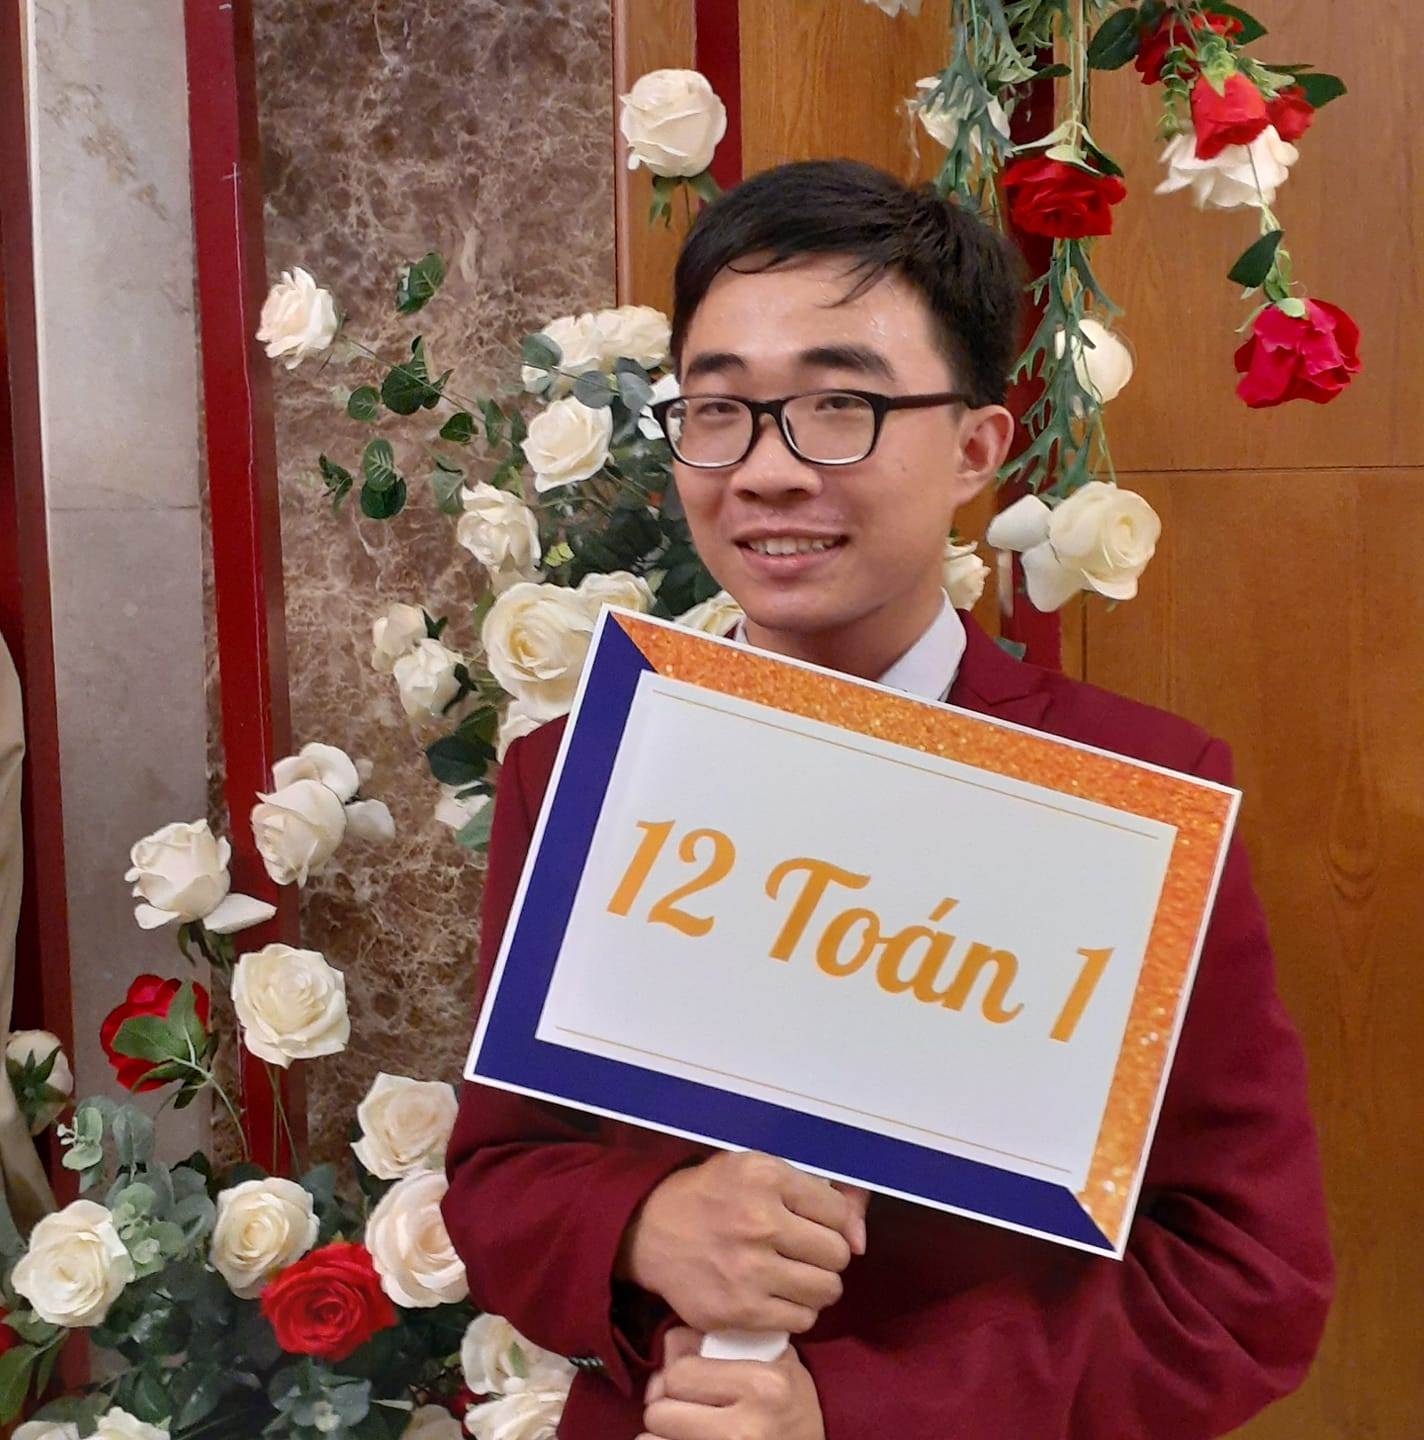
\includegraphics[height=3cm]{avt.jpg}
\end{minipage}
\vspace{-1em}
\section{Education}
\begin{cvcolumns}
    \cvcolumn[0.35]{~~~~~~~~~~~~~~~~Program}
    {
        \cvcolumncell {~\textit{ {{\textcolor{blue}{Bachelor}}}} (Information Technology)}
        \cvcolumncell {} 
    }
    \cvcolumn[0.38]{~~~~~~~~~~~~~Institution/Board}
    {
        \cvcolumncell{University of Science, Vietnam National University Ho Chi Minh City}
        \cvcolumncell{\textit{~~~~~~~~~~~~~~~~~~~~~Ho Chi Minh City, Vietnam}}
    }
    
    \cvcolumn[0.08]{~~~GPA}
    {
        \cvcolumncell{\textbf{~~~~8.89/10 (current)} }
        \cvcolumncell{}
    }
      
    \cvcolumn{~~~~~~~~~~~~Year}
    {
        \cvcolumncell{~~~~~~~~~~2020 - now}
        \cvcolumncell{}
    }
\end{cvcolumns}
\vspace{-1em}

\section{Knowledge}
\cvlistitem{Data Structures and Algorithms}
\cvlistitem{Databases}
\cvlistitem{Computer Networks}
\cvlistitem{Combinatorics}
\cvlistitem{Probability and Statistics}
\cvlistitem{Linear Algebra}

\vspace{-1em}

\section{Technical Skills}
\cvlistitem{Programming Techniques}
\cvlistitem{Object-Oriented Programming}
\cvlistitem{Socket Programming}
\cvlistitem{Programming Languages: C, C++, Python, R}
\cvlistitem{Web Technologies: HTML, CSS, JavaScript (basic)}
\cvlistitem{Database System: Microsoft SQL Server}
\cvlistitem{Operating Systems: Windows, Linux (Ubuntu, Kubuntu)}
\cvlistitem{Jupyter Notebook}
\cvlistitem{{Tools:} {\LaTeX, Anaconda, Microsoft Office}}
\vspace{-1em}

%\section{Key Projects}
\cventry{IIT Madras}{(M.Tech / Guide: Prof. XXXX)}
{1. \textit{{\href{https://somelinks}{\textcolor{blue}{~Project 1}}}} }{Aug 20xx - April 20xx}{}{}
\cvlistitem{Correctly \textbf{classified} the Kaggle eye image dataset into different stages of DR and also \textbf{predicted} an eye image as \textbf{abnormal or normal with 94\% accuracy.}}
\cvlistitem{\textit{Keywords: CNN, DR, Kaggle, GPU, Python, Anaconda, Keras, Confusion Matrix}}
%\cvlistitem{Language(used): Python}
%\cvlistitem{Tools/Libraries (used): Anaconda (Spyder), GPU }

\vspace{2mm}
\cventry{Jalpaiguri Government Engineering College}{(B.Tech / Guide: Mrs. XXXX)}
{2. \textit{{\href{https://somelinks}{\textcolor{blue}{~Project 2}}} }}{Jan-May 20xx}{}{}
\cvlistitem{Developed a \textbf{web portal} for taking online examination.}
\cvlistitem{\textit{Keywords: LAMP stack (Linux-Apache-Mysql-PhpMyadmin), HTML, CSS, Php}}
%\cvlistitem{Language: HTML, PHP, MySql}
%\cvlistitem{Tools: PhpMyAdmin, Xampp, Abode Dreamweaver}

\vspace{2mm}
\cventry{Darjeeling Polytechnic}{(Diploma / Guide: Asst. Prof XXXX)}
{2. \textit{{\href{https://someLinks}{\textcolor{blue}{~Project 2}}} }}{Jan-May 20xx}{}{}
\cvlistitem{Developed an application which detected malware in windows systems. }
\cvlistitem{\textit{Keywords: VB, Visual Basic}}

%\cvlistitem{Language: VB}
%\cvlistitem{Tools: Visual Basic }
%\vspace{-1em}

\section{Course Projects}
%\cvlistitem{}

\cventry{HCMUS}{}
{\textit{\textcolor{blue}{PC Control via Email}}
}{May - June 2022}{}{}
\cvlistitem{A socket application (server - client) that allows users to control their PCs in a LAN via email.}
\cvlistitem{Language: Python.}
\cvlistitem{Role: Socket Programmer, Tester.}
\cvlistitem{Projects for Computer Networks.}
\cvlistitem{GitHub link: \href{https://github.com/vanloc1808/HCMUS-Computer-Networks-Projects/tree/main/Socket-Email}{\textcolor{red}{https://github.com/vanloc1808/HCMUS-Computer-Networks-Projects/tree/main/Socket-Email}}}

\cventry{HCMUS}{}
{\textit{\textcolor{blue}{Favorite Place}}
}{May 2022}{}{}
\cvlistitem{A socket client $-$ server application for mananing favorite places.}
\cvlistitem{GUI uses \href{https://docs.python.org/3/library/tkinter.html}{\textcolor{red}{tkinter library}}.}
\cvlistitem{Language: Python.}
\cvlistitem{Role: Client Developer and GUI Designer.}
\cvlistitem{Projects for Computer Networks.}
\cvlistitem{GitHub link: \href{https://github.com/vanloc1808/HCMUS-Computer-Networks-Projects/tree/main/Socket-Place}{\textcolor{red}{https://github.com/vanloc1808/HCMUS-Computer-Networks-Projects/tree/main/Socket-Place}}}

\cventry{HCMUS}{}
{\textit{\textcolor{blue}{Research about Hidden Markov Model}}
}{April - May 2022}{}{}
\cvlistitem{A project for researching about Hidden Markov Model, includes: its theory, implementaion and application.}
\cvlistitem{Language: \LaTeX and Python with Jupyter Notebook.}
\cvlistitem{Role: Theory researcher, collaborative implementer.}
\cvlistitem{Projects for Applied Mathematics and Statistics.}
\cvlistitem{GitHub link: \href{https://github.com/vanloc1808/HCMUS-Applied-Maths-and-Statistics-Projects/tree/main/Project-2}{\textcolor{red}{https://github.com/vanloc1808/HCMUS-Applied-Maths-and-Statistics-Projects/tree/main/Project-2}}}

\cventry{HCMUS}{}
{\textit{\textcolor{blue}{Simple Data Description and Prediction}}
}{March - April 2022}{}{}
\cvlistitem{A project for data description and data prediction on a small set of data.}
\cvlistitem{Language: Python with Jupyter Notebook.}
\cvlistitem{Role: Collaborative Participant.}
\cvlistitem{Projects for Applied Mathematics and Statistics.}
\cvlistitem{GitHub link: \href{https://github.com/vanloc1808/HCMUS-Applied-Maths-and-Statistics-Projects/tree/main/Project-1}{\textcolor{red}{https://github.com/vanloc1808/HCMUS-Applied-Maths-and-Statistics-Projects/tree/main/Project-1}}}

\cventry{HCMUS}{}
{\textit{\textcolor{blue}{Simple Chess Game}}
}{October - December 2021}{}{}
\cvlistitem{A chess game implemented with the basic concepts of object-oriented programming.}
\cvlistitem{GUI uses \href{https://www.sfml-dev.org/}{\textcolor{red}{SFML library}}.}
\cvlistitem{Language: C++.}
\cvlistitem{Role: Main Developer.}
\cvlistitem{Projects for Object-Oriented Programming.}
\cvlistitem{GitHub link: \href{https://github.com/vanloc1808/HCMUS-OOP-Project-ChessGame}{\textcolor{red}{https://github.com/vanloc1808/HCMUS-OOP-Project-ChessGame}}}


\vspace{2mm}

\cventry{HCMUS}{}
{\textit{\textcolor{blue}{Search Engine}}
}{June 2021}{}{}
\cvlistitem{Search a string in a variety of text files, using TF/IDF.}
\cvlistitem{Language: C++.}
\cvlistitem{Role: Collaborative Developer.}
\cvlistitem{Projects for Arts of Programming.}
\cvlistitem{GitHub link: \href{https://github.com/mekanican/BigInteger}{\textcolor{red}{https://github.com/vanloc1808/HCMUS-AP-Project-SearchEngine}}}




\vspace{2mm}

\cventry{HCMUS}{}
{\textit{\textcolor{blue}{Big Integers}}
}{May 2021}{}{}
\cvlistitem{Implemented arithmetic and logic operations on big integers, $128$ bits or more.}
\cvlistitem{Language: C++}
\cvlistitem{Role: Collaborative Developer}
\cvlistitem{Projects for Arts of Programming}
\cvlistitem{GitHub link: \href{https://github.com/mekanican/BigInteger}{\textcolor{red}{https://github.com/mekanican/BigInteger}}}

\vspace{2mm}
%\vspace{-1em}

% \cventry{HCMUS}{}
% {\textit{\textcolor{blue}{Name}}
% }{Time}{}{}
% \cvlistitem{Description}
% \cvlistitem{Language: .}
% \cvlistitem{Role: }
% \cvlistitem{Projects for }
% \cvlistitem{GitHub link: \href{}{\textcolor{red}{}}}
\vspace{-1em}

\section{Online Courses }
\cvlistitem {Coursera: \\ 
\textit{\href{https://www.coursera.org/account/accomplishments/verify/PXKQ7TT2PJVS}{\textcolor{blue}{Python Project for Data Science}}} (June 2022),\\
\textit{\href{https://www.coursera.org/account/accomplishments/verify/7AHYRMCSQHH5}{\textcolor{blue}{Python for Data Science, AI \& Developmente}}} (June 2022),\\
\textit{\href{https://www.coursera.org/account/accomplishments/verify/Z3AQGSTYFCCX}{\textcolor{blue}{Data Science Methodology}}} (June 2022),\\
\textit{\href{https://www.coursera.org/account/accomplishments/verify/S2XX2YW466WU}{\textcolor{blue}{Tools for Data Science}}} (March 2022),\\
\textit{\href{https://www.coursera.org/account/accomplishments/verify/N43FVPW6X4DC}{\textcolor{blue}{What is Data Science?}}} (March 2022),\\
\textit{\href{https://www.coursera.org/account/accomplishments/verify/XRZ67WHD2B9F}{\textcolor{blue}{HTML, CSS, and Javascript for Web Developers}}} (March 2022),\\
\textit{\href{https://www.coursera.org/account/accomplishments/verify/6W53X97J2LGT}{\textcolor{blue}{Algorithmic Toolbox}}} (February 2022),\\
\textit{\href{https://www.coursera.org/account/accomplishments/verify/PXVGPATLHGDD}{\textcolor{blue}{Introduction to Git and GitHub}}} (February 2022),\\
\textit{\href{https://www.coursera.org/account/accomplishments/verify/CLD23RCC4TXN}{\textcolor{blue}{Writing in the Sciences}}} (September 2021)
}

% \cvlistitem {Jovian: \\ 
%\textit{\href{cert link}{\textcolor{blue}{course name}}} (time),\\
%\textit{\href{cert link}{\textcolor{blue}{course name}}} (time),\\
%\textit{\href{cert link}{\textcolor{blue}{course name}}} (time)\\
%}

\vspace{-1em}

\section{Achievements/Awards}

\cvlistitem {Successfully qualified 
\textit{{\href{https://someLinks}
        {\textcolor{blue}{UGC-NET}}}} (20xx),
\textit{{\href{https://someLinks}
        {\textcolor{blue}{SLET-NE Region}}}} (20xx),
\textit{{\href{https://someLinks}
        {\textcolor{blue}{WB-SET}}}} (20xx) and
\textit{{\href{https://someLinks}
        {\textcolor{blue}{GATE}}}} (20xx).}

\cvlistitem {Secured 3\textsuperscript{rd} rank out of 540 in 
\textit{{\href{https://someLinks}{\textcolor{blue}{Virtual Product Management Experience Project
}}}} conducted by Quollab (20xx).}

\cvlistitem {Competed in the  
\textit{{\href{https://someLinks}{\textcolor{blue}{Code To Japan Algorithms}}} and {\href{https://someLinks}{\textcolor{blue}{Code To Japan AI}}}} challenge, with overall 188/746 (20xx).}

\cvlistitem {Awarded as 
\textit{{\href{https://someLinks}{\textcolor{blue}{Star Teaching Assistant}}}} for contribution as a Teaching Assistant, by CSE Department, IIT Madras (20xx).}

\cvlistitem {Received the 
\textit{{\href{https://someLinks}{\textcolor{blue}{Certificate of Appreciation}}}} for donating blood, State Blood Transfusion Council, West Bengal (20xx).}


\cvlistitem {Secured 
\textit{{\href{https://someLinks}{\textcolor{blue}{2\textsuperscript{nd} in quiz competition}}}} in 
Rotary Youth Festival held by Rotary Club of Tura, Meghalaya (20xx).}

\cvlistitem {Secured 
\textit{{\href{https://someLinks}{\textcolor{blue}{1\textsuperscript{st} in quiz competition}}}} in 
Rotary Youth Festival held by Rotary Club of Tura, Meghalaya (20xx).}

\cvlistitem {Secured 
\textit{{\href{https://someLinks}{\textcolor{blue}{Consolation Prize}}}} in essay writing competition on topic \textit{Conservation of Natural resources} held by Soil Conservation Department, Meghalaya (20xx).}

\vspace{0.5em}

%Languages (Spoken/known): Assamese, Bengali, English, Garo, Hindi, Nepali. 
\vspace{-1em}

%\section{Online Courses Projects}
\cventry{Coursera}{}
{\textit{\textcolor{blue}{Analyzing Historical Stock/Revenue Data and Building a Dashboard}}
}{June 2022}{}{}
\cvlistitem{Extract the revenue data for Tesla and GameStop and build a dashboard to compare the price of the stock vs the revenue. }
\cvlistitem{Language: Python with Jupyter Notebook.}
\cvlistitem{Projects for \href{https://www.coursera.org/learn/python-project-for-data-science}{Python Project for Data Science}}
\cvlistitem{GitHub link: \href{}{\textcolor{red}{https://github.com/vanloc1808/Coursera-IBM-Data-Science-Professional-Certificate/blob/main/Course05.Python-Projects-for-Data-Science/Final-Assignment.ipynb}}}
\vspace{-1em}

%\section{Industrial Training}
\cventry{National Skill Development Corporation, Kolkata}{(B.Tech / Mentor: Mrs XXXX) }
{1. \textit{{\href{https://someLinks}{\textcolor{blue}{Employee Appraisal System}}}}   }{Dec 20xx - Jan 20xx}{}{}
\cvlistitem{Developed an application which computed the salary hike of an employee based on the performance rating.   }


\vspace{2mm}
\cventry{Bharat Sanchar Nigam Limited, Jalpaiguri}{(Diploma / Mentor: XXXXXX)}
{2.  \textit{{\href{https://someLinks}{\textcolor{blue}{Bharat Sanchar Nigam Limited (Networking)}}}}}{Oct-Nov 20xx}{}{}
\cvlistitem{Studied the working of landline phones and its architecture, in specified stream of Switching, OFC \& IT.}   

\vspace{-1em}

%\section{Course Work}
\cventry{IIT Madras}{(Core and electives)}{1. Key Courses}{August 20xx-April 20xx}{}{}

\cvlistitem{{Course}: Advanced Data Structures and Algorithms, Logic and Combinatorics for Computer Science, Theory and Applications of Ontology, Digital System Testing and Testable Design, Applied Cryptography, Non-linear Optimization}
\cvlistitem{{Lab}: Advanced Programming Languages in C++}
\vspace{-1em}


%\section{Positions of Responsibility}
\begin{itemize}
\item \textit{{\href{https://someLinks}
              {\textcolor{blue}{Mentor}}}} at Going Online As Leaders (GOAL) jointly initiated by Facebook India and MoTA - Govt. of India. (20xx-xx).

\item \textit{{\href{https://someLinks}{\textcolor{blue}{Teaching Assistant}}}} for Computational Engineering course, CSE Department, IIT Madras (Jan-May, 20xx).

\item \textit{{\href{https://someLinks}{\textcolor{blue}{Teaching Assistant}}}} at Computing Facility, CSE Department, IIT Madras (July-Nov, 20xx). 

\item \textit{{\href{https://someLinks}{\textcolor{blue}{Teaching Assistant}}}} at Library, CSE Department, IIT Madras (Jan-May, 20xx).

\item \textit{{\href{https://someLinks}{\textcolor{blue}{Teaching Assistant}}}} for Computational Engineering course, CSE Department, IIT Madras (July-Nov, 20xx).
\end{itemize}
\vspace{-1em}

%\section{Workshops}
\cvlistitem {Participated in the webinar, 
\textit{{\href{https://someLinks}{\textcolor{blue}{Foundations of Vedic Mathematics}}}} conducted by SSNU, Tamil Nadu (20xx).}

\cvlistitem {Participated in the webinar on 
\textit{{\href{https://someLinks}{\textcolor{blue}{NBA Accreditation \& Role of Stakeholders in the light of National Education Policy (2020)}}}}, organized by Women's polytechnic, Tripura in association with NITTTR, Kolkata (20xx).}

\cvlistitem {Participated the 
\textit{{\href{https://someLinks}{\textcolor{blue}{International Youth Web-Conclave on Vasudhaiva Kutumbakam}}}}, jointly organized by Sixth Sense Foundation, Shree Sisters, Kongunadu Arts and Science College, Sri Sarada Niketan College of Science for Women and Global International School (Nov 20xx).}

\cvlistitem {Attended the workshop on 
\textit{{\href{https://someLinks}{\textcolor{blue}{Program for Aspiring College Teachers (PACT)}}}}, conducted by TLC, IIT Madras (20xx).}
\vspace{-1em}



%\section{Others}
\cvlistdoubleitem{Hobbies: Travelling, Cooking, Learning languages}{Languages: Bengali, Hindi, Assamese, Nepali, Garo.}
\vspace{-1em}

%\section{Declaration}
{I do hereby declare that all the details furnished above are true to the best of my knowledge and belief.}\\

{Place: Somewhere, State (Country)\hspace{25em} (Full Name)}\\
{Date: 18th Aug, 20xx}
\vspace{5mm}

\end{document}


%% end of file `template.tex'.
